%% ----------------------------------------------------------------
%% Progress.tex
%% ---------------------------------------------------------------- 

\documentclass[oneside]{ecsproject}     % Use the Project Style
\usepackage{titlesec}
\usepackage{makecell}
\usepackage{pgfgantt}
\usepackage{pdflscape}
\usepackage[outputdir=output]{minted}

\titleformat{\chapter}
  {\normalfont\huge\bfseries}{\ \thechapter.}{18pt}{\huge}
\graphicspath{{figures/}}   % Location of your graphics files
\usepackage{natbib}            % Use Natbib style for the refs.
\hypersetup{colorlinks=false}   % Set to false for black/white printing

\newcommand{\vref}[1]{\textit{\hyperref[#1]{#1}}}
\newcommand{\lref}[1]{Listing~\ref{#1}}
\newcommand{\rref}[1]{\textit{\hyperref[#1]{#1}}}

\begin{document}
\frontmatter
\title      {Folidity - Safe Functional Smart Contract Language}
\authors    {\texorpdfstring
             {\href{mailto:gn2g21@soton.ac.uk}{German Nikolishin}}
             {German Nikolishin}
            }
\addresses  {\groupname\\\deptname\\\univname}
\date       {\today}
\subject    {}
\keywords   {}
\supervisor {\texorpdfstring
            {\href{mailto:gn2g21@soton.ac.uk}{Prof. Vladimiro Sassone}}
            {Prof. Vladimiro Sassone}
}
\examiner   {TBD}
\degree     {BSc Computer Science}
\maketitle

\begin{abstract}
  This paper addresses the long-lasting problem involving the exploits of Smart Contract vulnerabilities.
  There are tools, such as in the formal verification field and alternative Smart Contract languages, that
  attempt to address these issues. However, neither approach has managed to combine
  the static formal verification and the generation of runtime assertions. 
  Furthermore, this work believes that implicit hidden state transition is the root cause
  of security compromises. In light of the above, we introduce Folidity, a safe functional Smart Contract language
  with a unique approach to reasoning about the modelling and development of Smart Contract systems.
  Folidity features explicit state transition checks, a model-first approach, and built-in formal verification
  tooling.
\end{abstract}

\chapter{Statement of Originality}
\small
\begin{itemize}
    \item I have read and understood the \href{http://ecs.gg/ai}{ECS Academic Integrity} information and the University’s \href{https://www.southampton.ac.uk/quality/assessment/academic_integrity.page}{Academic Integrity Guidance for Students}.
    
    \item I am aware that failure to act in accordance with the \href{http://www.calendar.soton.ac.uk/sectionIV/academic-integrity-regs.html}{Regulations Governing Academic Integrity} may lead to the imposition of penalties which, for the most serious cases, may include termination of programme.

    \item I consent to the University copying and distributing any or all of my work in any form and using third parties (who may be based outside the EU/EEA) to verify whether my work contains plagiarised material, and for quality assurance purposes.
\end{itemize}

\textbf{You must change the statements in the boxes if you do not agree with them.}

We expect you to acknowledge all sources of information (e.g. ideas, algorithms, data) using citations. You must also put quotation marks around any sections of text that you have copied without paraphrasing. If any figures or tables have been taken or modified from another source, you must explain this in the caption and cite the original source. 

\footnotesize
\begin{tabular}{|p{\textwidth}|}
\hline
\textbf{I have acknowledged all sources, and identified any content taken from elsewhere.} \\
\hline
\end{tabular}
\small

 If you have used any code (e.g. open-source code), reference designs, or similar resources that have been produced by anyone else, you must list them in the box below. In the report, you must explain what was used and how it relates to the work you have done.

\footnotesize
\begin{tabular}{|p{\textwidth}|}
\hline
\textbf{I have not used any resources produced by anyone else.} \\
\hline
\end{tabular}
\small

 You can consult with module teaching staff/demonstrators, but you should not show anyone else your work (this includes uploading your work to publicly-accessible repositories e.g. Github, unless expressly permitted by the module leader), or help them to do theirs. For individual assignments, we expect you to work on your own. For group assignments, we expect that you work only with your allocated group. You must get permission in writing from the module teaching staff before you seek outside assistance, e.g. a proofreading service, and declare it here.

\footnotesize
\begin{tabular}{|p{\textwidth}|}
\hline
\textbf{I did all the work myself, or with my allocated group, and have not helped anyone else.} \\
\hline
\end{tabular}
\small

 We expect that you have not fabricated, modified or distorted any data, evidence, references, experimental results, or other material used or presented in the report. You must clearly describe your experiments and how the results were obtained, and include all data, source code and/or designs (either in the report, or submitted as a separate file) so that your results could be reproduced. 

\footnotesize
\begin{tabular}{|p{\textwidth}|}
\hline
\textbf{The material in the report is genuine, and I have included all my data/code/designs. } \\
\hline
\end{tabular}
\small

 We expect that you have not previously submitted any part of this work for another assessment. You must get permission in writing from the module teaching staff before re-using any of your previously submitted work for this assessment.

\footnotesize
\begin{tabular}{|p{\textwidth}|}
\hline
\textbf{I have not submitted any part of this work for another assessment.} \\
\hline
\end{tabular}
\small

 If your work involved research/studies (including surveys) on human participants, their cells or data, or on animals, you must have been granted ethical approval before the work was carried out, and any experiments must have followed these requirements\textit{.} You must give details of this in the report, and list the ethical approval reference number(s) in the box below.

\footnotesize
\begin{tabular}{|p{\textwidth}|}
\hline
\textbf{My work did not involve human participants, their cells or data, or animals.} \\
\hline
\end{tabular}
\small

 \normalsize

\tableofcontents
% \listoffigures
% \listoftables
% \lstlistoflistings
% \listofsymbols{ll}{$w$ & The weight vector}
\mainmatter

%% ----------------------------------------------------------------

\chapter{Introduction}

The concept of "smart contract" [SC] was first coined by Nick Szabo as a computerised transaction protocol \cite{nz_sc}.
He later defined smart contracts as observable, verifiable, privity-applicable, and enforceable programs. \cite{nz_sc_bb}.
In other words, smart contracts were envisioned to inherit the natural properties of traditional "paper-based" contracts.

In 2014 SCs were technically formalised at the protocol level by Dr. Gavin Wood as an arbitrary program
written in some programming language (Solidity) and executed in the blockchain's virtual machine of Ethereum.\cite{eth_yellow_paper}.

Ethereum Virtual Machine (EVM) iterated over the idea of Bitcoin Scripting, allowing developers to deploy general-purpose, Turing-Complete
programs that can have their own storage, hence the state, written in Solidity\cite{solidity_docs}. This enabled sophisticated applications that grew beyond
the simple funds transfers among users.

Overall, SC can be summarised as an \textit{immutable}, \textit{permissionless}, \textit{deterministic} computer programs 
that are executed as part of state transition in the blockchain system. 

After a relatively short time, SCs have come a long way and allowed users to access different online services in a completely trustless and decentralised way.
The applications have spanned financial, health, construction\cite{cad_blockchain}, and other sectors. 

\chapter{Security and Safety of Smart Contracts}

\section{Overview}

With the increased adoption of decentralised applications (DApps) and total value locked in DApps, 
there have been numerous attacks focused on extracting funds from SCs. 
Due to the permissionless nature of SCs, the most common attack vector exploits the mistakes in the SC's source code.
Specifically, the attacker can not tamper with the protocol code due to consensus mechanisms.
Instead, they can interact with the publicly accessible parameters and interfaces to force the SC into an unexpected state, essentially gaining partial control of it.

A notorious example is the DAO hack when hackers exploited unprotected re-entrance calls to withdraw \textbf{\$50 million worth of ETH}. 
This event forced the community to hard-fork the protocol to revert the transaction, provoking a debate on the soundness of the action \cite{the_dao}.

Another less-known example is the "King of the Ether" attack, which was caused by the unchecked low-level Solidity \texttt{send} call to transfer funds to a contract-based wallet \cite{king_of_the_ether}.
The "King of the Ether Throne" contract could not recognise the failed transaction on the wallet side. Instead, the contract proceeded with the operation, incorrectly mutating its internal state.

Other issues involve the \textit{safety} and \textit{liveness} of SCs. 
The term \textit{safety} is used to describe the \textit{functional safety} and \textit{type safety}. It is often used interchangeably with the \textit{security} of code
as compromising the former affects the latter. When talking about \textit{liveness}, we describe the business logic of a DApp, particularly whether it transitions into the expected new state.

\textit{Safety} and \textit{liveness} can be compromised due to the programmer's mistakes in the source code that can result in the SC entering the terminal in an unexpected state
preventing users from interacting with it\cite{ondo_report}.


\section{Vulnerability classification}

There has been an effort in both academia and industry to classify common vulnerabilities 
and exploits in SCs in blockchain systems \cite{owasp}\cite{stefano}\cite{atzei_survey}. 
Some of the work has been recycled by bug bounty platforms, growing the community of auditors
and encouraging peer-review of SCs through the websites such as \textit{Code4rena}\footnote{https://code4rena.com}, \textit{Solodit}\footnote{https://solodit.xyz},
and many others.

Analysing the work mentioned above, SC vulnerabilities can be categorised into the six general groups outlined in \tref{Table:classification}.

\begin{table}[!htb]
  \centering
  \begin{tabular}{ccc}
  \toprule
  \textbf{Code} & \textbf{Title} & \textbf{Summary}\\
  \midrule
  \textit{SCV1}\label{SCV:1} & \makecell{Timestamp\\manipulation} & \makecell{\\Timestamp used in \\control-flow, randomness and storage,\\can open an exploit due to an ability\\for validator to manipulate the timestamp}\\\\
  \hline
  \textit{SCV2}\label{SCV:2} & \makecell{Pseudo-randomness} & \makecell{\\Using block number, block hash,\\block timestamp\\are not truly random generated parameters,\\and can be manipulated by the adversary validator}\\\\
  \hline
  \textit{SCV3}\label{SCV:3} & \makecell{Invalidly-coded\\states} & \makecell{\\When coding business logic,\\ control-flow checks\\can be incorrectly coded resulting the SC\\entering into invalid state}\\\\
  \hline
  \textit{SCV4}\label{SCV:4} & \makecell{Access Control\\exploits} & \makecell{\\This is a more broad categorisation of vulnerabilities.\\It occurs when an adversary calls a restricted function.\\This is specifically present in\\\textit{upgradeability} and \textit{deleteability} of SCs}\\\\
  \hline
  \textit{SCV5}\label{SCV:5} & \makecell{Arithmetic operations} & \makecell{\\SCs are suspected to the same arithmetic bugs\\as classic programs.\\Therefore, unchecked operations can result\\in underflow/overflow or deletion by zero}\\\\
  \hline
  \textit{SCV6}\label{SCV:6} & \makecell{Unchecked externall\\calls} & \makecell{\\Unchecked re-entrant, forward, delegate\\calls can result in the contract\\entering into unexpected state}\\\\
  \bottomrule
  \end{tabular}
  \caption{Classification of SC vulnerabilities}
  \label{Table:classification}
\end{table}

\section{Setting the scene} \label{Section:Scene}

Even with the raised awareness for the security and safety of SCs, recent reports from \textit{Code4rena} still show \vref{SCV:3}, \vref{SCV:4} and \vref{SCV:5}
commonly present in the recent audit reports\cite{arcade_report}\cite{ondo_report}\cite{centrifuge_report}.

In particular, in \cite{centrifuge_report}, a relatively simple calculation mistake resulted in other SC users being unable to withdraw their funds.

It can be seen that SC Vulnerabilities illustrated in \tref{Table:classification} are still evident in modern SCs, resulting in opening them up to vulnerabilities of different severity levels.
Looking at the mentioned reports, there is little consensus about the weight of each vulnerability.
Therefore, we can not classify any particular vulnerability as more severe than the other as it solely depends on the context in the code it is present.
Furthermore, it has been realised that additional tooling or alternative SCLs need to be discovered to minimise the exposure of SC code to the earlier-mentioned vulnerabilities.

\chapter{Current Solutions}

\section{Overview}

Different solutions have been presented to mitigate the consistency in the presence of vulnerabilities and programmer mistakes. 
We can generally categorise them into two groups: safe SCLs, which allow users to write safe and secure code, particularly described in \cref{Chapter:SCL}, 
and formal verification tools used alongside traditional SCLs presented in \cref{Chapter:FVT}.

This chapter reviews both categories of tools, allowing us to evaluate their effectiveness in correlation to usability,
aiming to provide a concise framework to analyze and work with the SC tools dedicated to producing
error-proof DApps. 

% \section{Solidity: the good and the bad}

% Before we begin analysing existing solutions, we should introduce the first and most popular SCL, Solidity\cite{sc_survey}\cite{solidity_docs}.
% Solidity has paved the way for SC development and has become a de facto standard in the blockchain space. We will later discover a lot of similarities with Solidity in other SCLs.
% Understanding how Solidity works will enable us to understand its limitations and how other SCLs and toolings try to address them.

% Solidity is a domain-specific, object-oriented\footnote{It is also often referred to as \textit{contract-oriented}. We will use these terms interchangeably.}, statically typed, compiled
% programming language\cite{solidity_docs}.

% Looking at the \lref{Listing:solidity}, we can identify some similarities with the OOP languages and C-like syntax.
% In particular, Solidity shares visibility keywords on lines \textit{6} and \textit{20}, variable declarations, and methods.
% Noting the differences, Solidity has blockchain-specific data types such as \textit{address}, which intuitively represents an address on the system.
% Importantly, functions have to be declared \textit{public} in order to be callable externally by the user or other contracts.
% We can also see the event declaration on the line \textit{7}, which allows EVM to log an action on the system to be accessed by the client.
% Solidity also offers specific functions, called modifiers, that allow for a change of behaviour of the function it is used on\cite{solidity_docs}.
% Finally, \textit{view} keyword allows that the function does not modify the state and only reads from it.
% Other specification details are omitted as they touch upon more EVM-specific functionality.

% It is evident from the listing the similarity of Solidity with other C-inspired systems languages that reduces
% the learning curve and makes it more appealing for developers to pick up.
% The simplicity of syntax also enables clarity in reading the code and auditing it. The imperative and object-oriented style
% provides additional familiarity for developers, allowing them to think of an individual contract as a class object.

% \begin{listing}
% \begin{minted}[linenos]{c}
% // SPDX-License-Identifier: GPL-3.0
% pragma solidity >=0.7.0 <0.9.0;

% contract Owner {

%     address private owner;
%     event OwnerSet(address indexed oldOwner, address indexed newOwner);

%     modifier isOwner() {
%         require(msg.sender == owner, "Caller is not owner");
%         _;
%     }

%     constructor() {
%         console.log("Owner contract deployed by:", msg.sender);
%         owner = msg.sender;
%         emit OwnerSet(address(0), owner);
%     }

%     function changeOwner(address newOwner) public isOwner {
%         emit OwnerSet(owner, newOwner);
%         owner = newOwner;
%     }

%     function getOwner() external view returns (address) {
%         return owner;
%     }
% }
% \end{minted}
% \caption{Simple Solidity contract}
% \label{Listing:solidity}
% \end{listing}

% On the other side, programming in Solidity comes with similar challenges as its parents. 
% Developers need to be aware of its operations on memory and storage when designing complex storage applications, 
% how the execution stack is handled at the VM level, 
% and implications on using unchecked arithmetic operations \vref{SCV:5}.
% Additionally, the vulnerabilities listed in \tref{Table:classification} 
% has been mainly composed of Solidity SC exploits.
% Moreover, the immutable nature of SCs restricts the iterative approach in development,
% posing an even greater responsibility on developers to model and design programs carefully.
% This is where formal verification tools have found strong applications.

\section{Formal Verification Tools} \label{Chapter:FVT}
\paragraph*{}
Formal verification describes the assessment of the correctness of a system concerning a formal specification\cite{eth_formal_verification}. 
The specification is usually described
in terms of verified models using mathematical proofs. There are multiple ways to verify a program formally focused on specific parts. \textit{Model checking} utilises propositional logic 
to verify the mathematical abstractions of the system. \textit{Theorem proving} involves verifying
relations between the model and the statements about the system. Finally, \textit{symbolic execution} focuses
on the execution of the program using symbolic values instead of concrete values\cite{eth_formal_verification}.
Different tools utilise different combinations of methods mentioned above.

KEVM\footnote{https://jellopaper.org/index.html} is a tool that provides an executable semantics of EVM using $\mathbb{K}$ framework. 
It uses reachability logic to reason symbolically about the system\cite{kevm}. KEVM is a powerful tool that operates at the EVM bytecode level.
Specifically, SC developers are required to write a specification in a separate file that is checked against the compiled EVM bytecode of the SC.
Whilst this provides more fine-grained assurance of the safety and correctness, it requires specialised knowledge of the $\mathbb{K}$ framework and EVM
semantics, hence significantly increasing the development time.

The other interesting tool is Dafny\footnote{https://dafny.org/latest/DafnyRef/DafnyRef}. Dafny is a general-purpose tool that checks inputs in any language 
using Hoare-logic and high-level annotations. Although Dafny offers compilation to some system languages, Solidity is not yet a supported target. 
Notably, work in the field suggests that the Dafny can be an effective and easy-to-use tool to produce a formal specification\cite{dafny_deductive}.
The syntax resembles a traditional imperative style and is substantially easier to learn and understand than KEVM.

Some tools can be used alongside Solidity code, such as Scribble\footnote{https://docs.scribble.codes/}. 
Scribble enables developers to provide formal specifications of functions inside docstrings seamlessly integrating with existing Solidity code. 
It offers VS Code extensions and is actively maintained by Consensys. 
The trade-off is the limited expressiveness in comparison with KEVM and Dafny.

Finally, experiments have been conducted to verify SC without any formal annotations. 
In particular, VeriSmart focuses explicitly on ensuring arithmetic safety and preciseness in SCs\cite{so2019verismart}. 
However, VeriSmart fails to detect other types of errors, 
although an effort has been made to apply the verifier to more areas of SC\cite{azure}.

\paragraph*{}
Formal verification is a multi-disciplinary field offering multiple ways of reason about the systems. One of the actively researched topics
is bounded model verification\cite{SMBC}. Developers are required to reason about the programs as finite state machines (FSM).
This reasoning approach is more apparent in SC development since the state transition is at the core of blockchain execution.
Bounded model checking has been realised by only a few experimental projects such as Solidifier\cite{solidifer} and Microsoft\cite{azure}.
Both projects attempt to translate Solidity code to an intermediate modelling language, Boogie\cite{boogie}. Boogie then leverages
SMT solvers to find any assertion violations.

Overall, we can see that formal verification tools provide a robust way of ensuring the safety of SCs. 
While significant effort has been made in the field, it is evident that formal verification tools in SC development
attempt to compensate for Solidity's implicit state transitions and lack of \textit{implicit} safety.

\section{Safe Smart Contract Languages} \label{Chapter:SCL}

Multiple attempts have been made to address a flawed programming model of Solidity\cite{sc_survey}. Alternative SCLs aim to provide
built-in safety features in a type system, modelling, and function declaration to minimise the need for
external tooling. 

Some languages, such as Vyper\footnote{https://docs.vyperlang.org/en/latest/index.html}, strive for simplicity.
By stripping off some low-level features, Vyper minimises the developer's chances of misusing the dangerous operations.
It also provides overflow checking, signed integers, and other safe arithmetic operations. However, Vyper is still immature, 
and the recent bug in the compiler caused a massive re-entrancy exploit in the \textit{curve.fi} AMM protocol\cite{curve}.
Furthermore, Vyper still suffers from the same implicit state transition problem as Solidity.

% To address the problem, it has been realised that a functional programming style may be better for SC development due to
% an explicit approach to reason about a state transition. Although some small effort has been made to adapt Haskell, neither project received any long-term support. It is still worth looking at some of the languages that suggest novice approaches to development. 

Flint is an experiment language with protected calls and asset types\cite{flint}. Protected calls introduce a role-based access system
where the SC developer can specify the permitted caller to a message function. Another unique feature is array-bounded loops
that partially address the halting problem. Flint also addresses a state-transition problem by allowing developers to specify
all possible states in the contract. The message functions need to specify the state transition, which occurs explicitly.
The language provides a significant improvement in a modelling approach. However, it still lacks the modelling SC input data in terms
of constraints and invariants, and explicit state transition is still an optional feature that the developer can miss in using.

Another promising SCL reasons about SC development through dependent and polymorphic types\cite{idris}. It extends Idris\footnote{https://www.idris-lang.org} 
and makes the developer model the SC as part of a state transition function by adopting a functional programming style. Dependent types provide a more
fine-grained controller over the input and output data that flow through the SC functions. In particular, similar to Haskell, the language offers \textit{side-effects} 
functionality that resembles \textit{IO} monads in Haskell. The downside of the approach is that the syntax has become too cumbersome for other developers to learn. Thus,
it has been stated that the language does not strive for simplicity and sacrifices it for safety.


\section{Problem statement}

We can identify the positive trend in providing the safety of SCs.
Modern formal verification methods offer support to SC developers in ensuring that their code satisfies the requirements of the system, while
proposed SCL solutions offer runtime safety, minimising the need for the former.

However, there has been no effort to combine the two approaches into a single development process. Formal verification tools
focus on the validation of functional correctness and model consistency of a program at the compile time, whereas SCLs focus on data validation 
at the runtime. Recent work suggests that the improved optimisation of SMT solvers allows us to turn the formal model specification into 
the runtime assertions\cite{runtime_assert}. Furthermore, no effort has been made to minimise false negatives in SC formal modelling, 
even though the methods have been developed for traditional systems, such as Event-B\cite{event_b}.

%% ----------------------------------------------------------------

\chapter{Proposed Solution} \label{Chapter:Solution}

\section{Outline}

In light of the above, we believe there is a need for a solution that combines two approaches to allow SC developers to reason
about their program in terms of FSM models that can be verified at the compile time for functional correctness and model consistency,
and enable an automatic generation of invariants and constraints to validate the data at runtime.

We propose \textit{Folidity}, a safe smart contract language. Folidity will offer the model-first approach to the development process
while featuring the functional-first programming style. The language intends to offer a safe and secure-by-design approach to the programming, 
ensuring the developer is aware of any state transitions during execution.

The list of feature requirements has been comprised based on the vulnerabilities described in \tref{Table:classification}.

\begin{description}
  \item[1. Provide abstraction over timestamp]\label{Requirements:1} in response to \vref{SCV:1}. We are interested in the limited use of timestamps in SCs in favour of block number or another safe primitive.
  \item[2. Provide a safe interface for randomness]\label{Requirements:2} in response to \vref{SCV:2}. Folidity should also provide source of randomness through a standardised interface.
  \item[3. Enable model-first approach in development]\label{Requirements:3} in response to \vref{SCV:3}. Developers should reason about the storage in terms of models and how they are updated by events. 
This approach is inspired by the Event-B\cite{event_b} work, which can also be applied to SC development.
  \item[4. Explicit state checks at runtime]\label{Requirements:4} in response to \vref{SCV:3} and \vref{SCV:6}. Similar to \rref{Requirements:3}, SC developers should be aware of any state transitions
that update the state of the model. State transitions must happen explicitly and be validated at the runtime to guarantee \textit{liveness}.
  \item[5. Static typing]\label{Requirements:5} in response to \vref{SCV:3} and \vref{SCV:5}.
  \item[6. Polymorphic-dependent types]\label{Requirements:6} in response to \vref{SCV:3}. Polymorphic-dependent types should be part of a runtime assertion check 
during state transition and model mutation\footnote{\textit{Model mutation} and \textit{state transition} refer to the same process. They are used interchangeably}.
  \item[7. Role-based access]\label{Requirements: 7} in response to \vref{SCV:4}. 
All message functions that mutate the model should be annotated with the role-access header specifying which set of accounts is allowed to call it.
  \item[8. Checked arithmetic operations]\label{Requirements:8} in response to \vref{SCV:5}. 
All arithmetic operations should be checked by default, and the developer is responsible for explicitly specifying the behaviour during over/underflow, similar to Rust.
  \item[9. Enforced checked recursion or bounded loops]\label{Requirements:9} in response to \vref{SCV:3}.
Infinite loops should not be permitted, and any loops should generally be discouraged in favour of recursion. The recursion base case should be specified explicitly with appropriate invariants.
Bounded loops may be used but should be limited to list or mapping iterations.
\end{description}

As part of the language design, the SC building workflow is illustrated in \fref{Figure:compilation}

\begin{figure}[!htb]
  \centering
  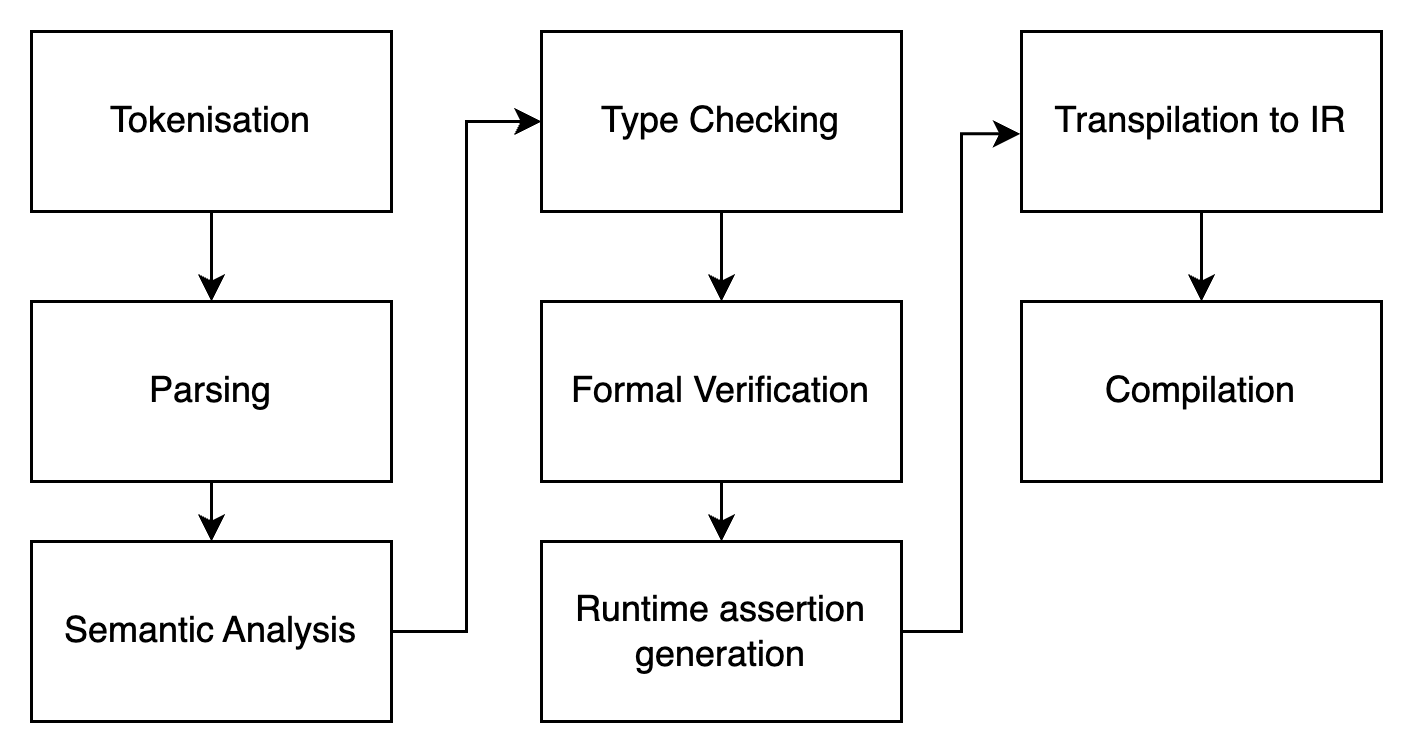
\includegraphics[width=10cm]{compilation.png}
  \caption{Build workflow}
  \label{Figure:compilation}
\end{figure}

As one of the core features of Folidity, formal verification is part of the build process.
Having verified the model consistency, invariants, and constraints, the program is considered safe to generate runtime assertions.

Another core feature is a pure computation context of the SC in Folidity. As illustrated in \fref{Figure:context:old},
state mutations to the contract storage and the global state (e.g. account balances) happen independently of each other. 
Folidity proposes a new execution model when a portion of a global state is \textit{embedded} into the local state of the SC 
as shown in \fref{Figure:context:transformed}. 

\begin{figure}[!htb]
  \centering
  \subfigure[Traditional execution context]{
    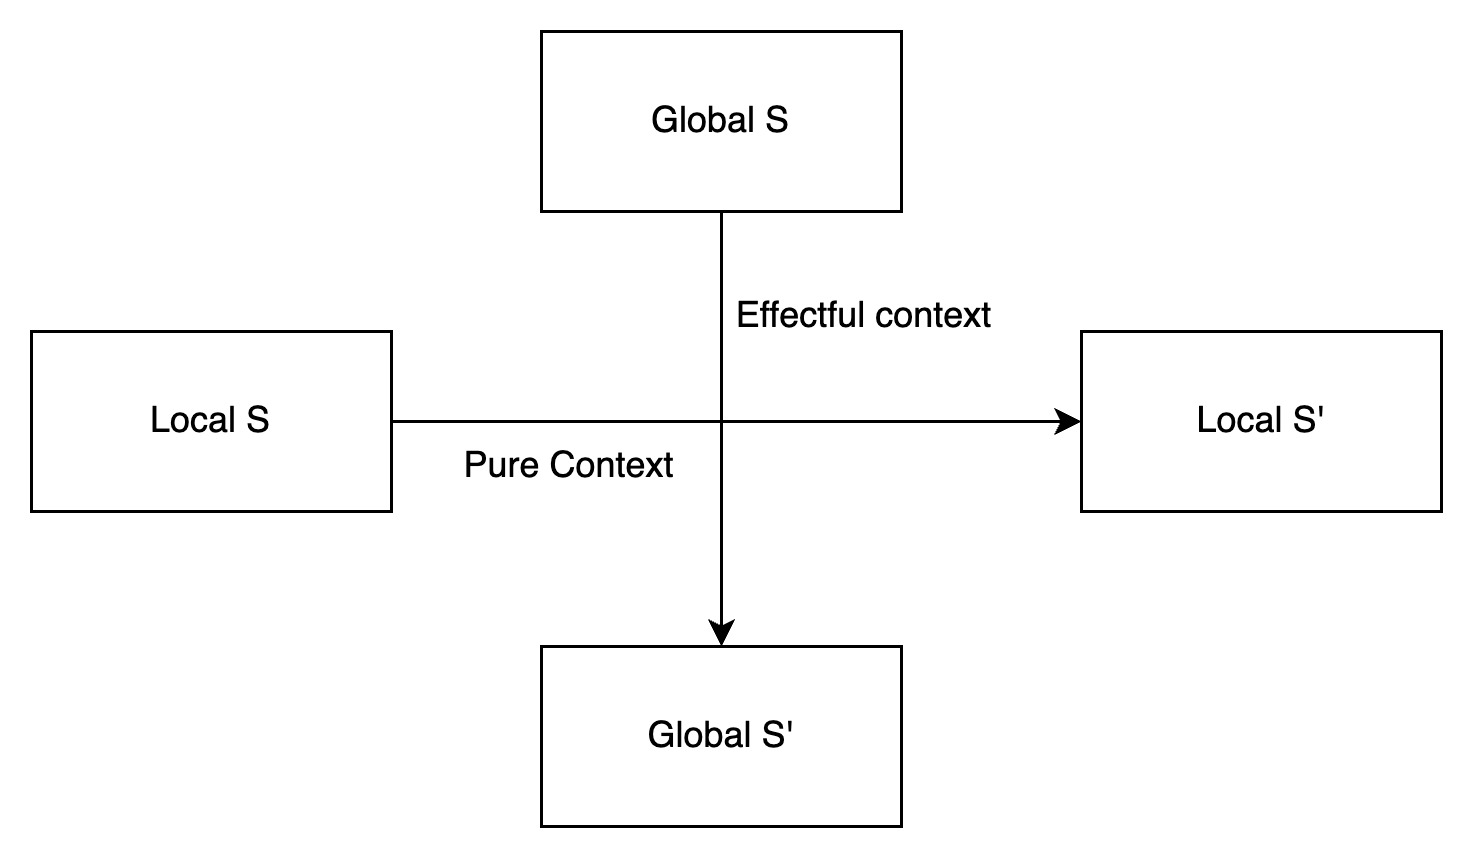
\includegraphics[width=7.5cm]{trad_context.png}
    \label{Figure:context:old}
  }
  \subfigure[Transfomed execution context]{
    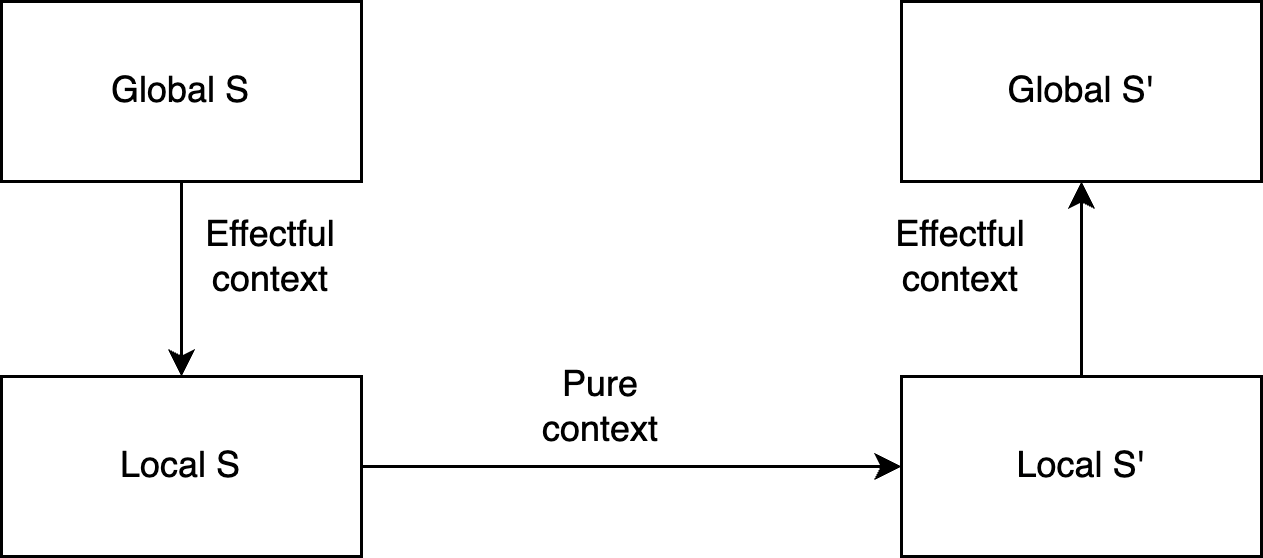
\includegraphics[width=7.5cm]{new_context.png}
    \label{Figure:context:transformed}
  }
  \caption{Changes to the execution context}
  \label{Figure:context}
\end{figure}


\newpage
\subsection{Model consistency: Simple example}

As an example of the theory behind model consistency in SCs, let's look at role-based access. Suppose:
\begin{itemize}
  \item $* = \{ \text{All addresses} \}$
  \item $M = \{ \text{Moderators of the system} \}$
  \item $A = \{ \text{Admins of the system} \}$
\end{itemize}

Then, we can model a role-based access hierarchy as 
\[ A \subseteq M \subseteq * \]

Subsequently, given the invariant for the system \textit{add\_mod(a: Address)} we can define following invariant:
\begin{equation*}
    \begin{gathered}
      i_0 := card(A) = 1 \\
      i_1 := card(M) = 5
    \end{gathered}
  \end{equation*}

And the invariant for the event:

$$
i_2 := c \in A
$$

Where $c$ - caller's address.

For the denoted event, suppose we mutate the model by adding an address to a set of admins:
\begin{equation*}
  A := A \cup \{a\}
\end{equation*}

Then, we can verify the model consistency for some state transition $S \to S'$ using propositional logic.

\begin{equation*}
  \begin{gathered} 
   \frac{(i_0 \wedge i_1 \wedge i_2 ) \rightarrow A \cup \{a\}, a \in *, c \in A}{A \cup \{a\}}
  \end{gathered}
\end{equation*}

However, as it can be seen, one of the premises violates the invariant, in particular:
\begin{equation*}
  \frac{card(A) = 1 \rightarrow A \cup \{a\}, a \in *}{A \cup \{a\}}
\end{equation*}.

In practice, the following error can be picked at the compile time by using symbolic execution of the code.
The other invariant, $i_2$, can be picked at the runtime by generating an appropriate assertion.

\section{Implementation}

The language will be implemented using Rust\footnote{https://www.rust-lang.org} due to its memory-safety guarantees and efficiency. 
Different parser-combinators alongside custom lexers are going to be used for the development of the parser. 
Folidity also requires SMT-solver for formal verification and generation of runtime assertions. In order to facilitate this functionality,
Z3\footnote{https://microsoft.github.io/z3guide} will be used since it also provides Rust bindings. It was debated to use Boogie, since it provides
a higher-level abstraction, but it was quickly discarded due to lack of documentation and increased development time.

As a target blockchain for the language, Algorand\footnote{https://developer.algorand.org} has been selected. 
Algorand is a decentralized blockchain platform designed for high-performance and low-cost transactions, 
utilising a unique consensus algorithm called Pure Proof-of-Stake to achieve scalability, security, and decentralisation\cite{algorand}.
One of the potential drawbacks of the language is increased complexity due to complex abstractions and additional assertions. 
EVM-based blockchains have varying costs for the execution, i.e. fees, that depend on the complexity of a SC. 
On the contrary, although Algorand has a limited execution stack, it offers fixed, low transaction fees.
Additionally, Algorand execution context explicitly executes in terms of state transition, which perfectly suits the paradigm of Folidity.
Finally, Algorand offers opt-in functionality and local wallet storage, allowing users to explicitly opt-in to use the SC.
This provides additional support in the role-based access control in Folidity.

As a target compilation language, Tealish\footnote{https://tealish.tinyman.org} has been chosen.
Although, Algorand offers Teal\footnote{https://developer.algorand.org/docs/get-details/dapps/avm/teal/} –
a low-level, stack-based programming language. Due to increased complexity, it is more realistic to use Tealish.
It offers the same access control to stack and storage while providing the developer with useful high-level abstractions.


\section{Scope}

As part of the development process, it has been decided to limit the scope to supporting only a single SC execution.
Cross-contract calls require extra consideration in design and development. Therefore, \vref{SCV:6} may not be fully addressed in the final report.
Additionally, optimisation of the execution is not considered relevant at this stage in favour of safety and simplicity.
Finally, Algorand offers smart signatures, a program that is delegated a signing authority\footnote{https://developer.algorand.org/docs/get-details/dapps/smart-contracts/smartsigs}.
As they operate in a different way from SCs, they are also outside the scope of this project.

\begingroup
\renewcommand{\cleardoublepage}{}
\renewcommand{\clearpage}{}
\chapter{Project Planning}
\endgroup

A significant groundwork in research of current solutions and their limitations has been done as illustrated by Gannt chart in \aref{Appendix:Gannt}.
Since the requirements have been composed, some progress has been made in the design of BNF grammar that will later pave the way for the development
of the parser. It is still possible to research more formal verification methods during the grammar design.

From the beginning of January, the first iteration of grammar should be completed, and the active development of the type checker and formal verifier should begin.


%% ----------------------------------------------------------------

\appendix

\chapter{Gannt Chart}
\begin{landscape}
  \begin{figure}[tbp]
      \centering
      \begin{ganttchart}[y unit title=0.5cm,
      y unit chart=0.5cm,
      vgrid,hgrid,
      % title label anchor/.style={below=-1.6ex},
      % title left shift=.05,
      % title right shift=-.05,
      title height=1.5,
      progress label text={$\displaystyle #1 \% $},
      bar height=0.8,
      % group right shift=0,
      group top shift=.8,
      ]{1}{30}
      %labels
      \gantttitle{\bf{Month}}{30} \\ \\
      \gantttitle{October}{4} 
      \gantttitle{November}{4} 
      \gantttitle{December}{4} 
      \gantttitle{January}{4} 
      \gantttitle{February}{4} 
      \gantttitle{March}{4}
      \gantttitle{April}{4}
      \gantttitle{May}{2} \\
      %tasks
      \ganttgroup[progress=100]{Overview of SC vulnerabilities}{1}{9} \\
      \ganttbar[progress=100]{Common smart contract exploits}{2}{7} \\
      \ganttbar[progress=100]{Survey of SC languages}{3}{8} \\
      \ganttbar[progress=100]{Formal verification analysis}{6}{9} \\
      \ganttbar[progress=100]{Evaluation of current solutions and issues}{6}{8} \\ \\
  
      \ganttmilestone{Progress Report}{9} \\
  
      \ganttgroup[progress=22.5]{The design of the proposed solution}{7}{14} \\
      \ganttbar[progress=60]{Requirements}{7}{8} \\
      \ganttbar[progress=30]{BNF Grammar}{7}{9} \\
      \ganttbar[progress=0]{Sample programs}{9}{12} \\
      \ganttbar[progress=0]{Brief evaluation of the BNF grammar}{12}{14} \\ \\
  
      \ganttgroup[progress=0]{Implementation}{12}{24} \\
      \ganttbar[progress=0]{Syntax}{12}{14} \\
      \ganttbar[progress=0]{Type Checker}{15}{18} \\
      \ganttbar[progress=0]{Evaluator}{18}{24} \\
      \ganttbar[progress=0]{Model Checker}{18}{21} \\
      \ganttbar[progress=0]{Functional correctness checker}{20}{23} \\ \\
  
      \ganttgroup[progress=0]{Evaluation}{23}{28} \\ 
      \ganttbar[progress=0]{Testing}{23}{26} \\
      \ganttbar[progress=0]{Safety evaluation}{27}{27} \\
      \ganttbar[progress=0]{Overview of sample solutions}{27}{27} \\
      \ganttbar[progress=0]{Future work}{28}{28} \\ \\
  
      \ganttmilestone{Submission Deadline}{28}
      %relations 
  
      \end{ganttchart}
      \caption{Gantt Chart}
      \label{Appendix:Gannt}
  
  \end{figure}
  \end{landscape}

%% ----------------------------------------------------------------


\backmatter
\bibliographystyle{unsrt}
\bibliography{ECS}
\end{document}
%% ----------------------------------------------------------------
